\documentclass[oneside, a4paper, 12pt]{memoir}

\usepackage[utf8]{inputenc}
\usepackage[usenames,dvipsnames,svgnames,table]{xcolor}
\usepackage[marginparwidth=28mm]{geometry}
\usepackage[pdftex]{graphicx}
\usepackage{tikz}

\usepackage{filecontents}
\usepackage[T1]{fontenc}
\usepackage[UKenglish]{babel}
\usepackage{newpxtext,newpxmath}
\usepackage[babel=true]{csquotes}
\usepackage[round]{natbib}
\usepackage[colorinlistoftodos]{todonotes}
\usepackage{comment}
\usepackage{tikz}
\usetikzlibrary{arrows,automata}
\usepackage{ccaption}

% Logos
\newcommand{\ulb}{
\includegraphics[scale=1.1]{PageDeGarde_MFE/logo_ULB2.pdf}}
\newcommand{\polytech}{
\includegraphics[scale=0.35]{PageDeGarde_MFE/logo_polytech_FR.pdf}}

% Polices
\definecolor{ULBblue}{rgb}{0,0.2196,0.5765}
\newcommand{\fontTitle}{\sffamily \Huge\selectfont \color{ULBblue}}
\newcommand{\fontSubtitle}{\sffamily \LARGE \selectfont \color{ULBblue}}
\newcommand{\fontText}{\sffamily \selectfont}
\newcommand{\fontColor}{\sffamily \selectfont \color{ULBblue}}

% Titre
\newcommand{\titleA}{\fontTitle{Human - Robots Swarms Interaction}} % Titre identique au titre remis au secrétariat
%\newcommand{\titleB}{\fontTitle{Deuxième ligne de titre du mémoire}} % (dans la langue de rédaction a priori)
% Sous-titre
\newcommand{\subtitleA}{\fontSubtitle{An Escorting Robot Swarm that Diverts a Human}}
\newcommand{\subtitleB}{\fontSubtitle{away from Dangers (s)he cannot perceive.}}
% Titre du diplôme
\newcommand{\diplomaA}{\fontText{Mémoire présenté en vue de l’obtention du diplôme}} % A laisser en Français
\newcommand{\diplomaB}{\fontText{d'Ingénieur Civil en Informatique à finalité Intelligence Computationnelle}}

% Etudiant
\newcommand{\student}{\textbf{\sffamily \large Anthony Debruyn}}

% Supervision
\newcommand{\promAa}{\fontColor{Directeur}}
\newcommand{\promAb}{\fontText{Professeur Mauro Birattari}}
\newcommand{\promBa}{\fontColor{Co-Promoteur}}
\newcommand{\promBb}{\fontText{Professeur Marco Dorigo}}
\newcommand{\promCa}{\fontColor{Superviseur}}
\newcommand{\promCb}{\fontText{Gaëtan Podevijn, AndreaGiovanni Reina}}
\newcommand{\deptA}{\fontColor{Service}}
\newcommand{\deptB}{\fontText{IRIDIA}}

% Année académique
\newcommand{\yearA}{\fontColor{Année académique}}
\newcommand{\yearB}{\fontText{2014 - 2015}}

%%%%%%%%%%%%%%%%%%%%%%%%%%%%%%%%%%%%%%%%%%%%%%%%%%%%%%%
% MY NEW COMMANDS
%%%%%%%%%%%%%%%%%%%%%%%%%%%%%%%%%%%%%%%%%%%%%%%%%%%%%%%

\newcommand{\quoto}[2]{
\begin{quotation}
\textit{\enquote{#1} - #2}
\end{quotation}
}

\newcommand{\quot}[1]{\textit{\enquote{#1}}}


\newcommand{\epuck}[3][0] % [angle]{x}{y} avec angle optionel
{
	\draw [very thick, fill=white] (#2,#3) circle [radius=0.5];
	\draw [very thick, rotate around={#1:(#2,#3)}] (#2-0.25,#3-0.433) -- (#2,#3+0.45) -- (#2+0.25,#3-0.433);
}

\newcommand{\epuckred}[3][0] % [angle]{x}{y} avec angle optionel
{
	\draw [very thick, fill=white] (#2,#3) circle [radius=0.5];
	\draw [red, very thick, rotate around={#1:(#2,#3)}] (#2-0.25,#3-0.433) -- (#2,#3+0.45) -- (#2+0.25,#3-0.433);
}

\newcommand{\human}[3][0] % [angle]{x}{y}
{
	\draw [line width=1.5pt, rotate around={#1:(#2,#3)}] (#2,#3+1) -- (#2-0.866,#3-0.5) -- (#2+0.866,#3-0.5) -- cycle;
	\draw (#2,#3) node[scale=2, rotate around={#1:(#2,#3)}]{H};
}


\let\oldCaption\caption
\renewcommand{\caption}[2]{
\oldCaption[#1]{{\small\sffamily\bfseries #1:} #2}
}

%%%%%%%%%%%%%%%%%%%%%%%%%%%%%%%%%%%%%%%%%%%%%%%%%%%%%%%
% NEW STYLES
%%%%%%%%%%%%%%%%%%%%%%%%%%%%%%%%%%%%%%%%%%%%%%%%%%%%%%%

\captiondelim{ -- }
\captionnamefont{\small\sffamily\bfseries}
\captiontitlefont{\small\sffamily}
\precaption{\rule{\linewidth}{0.4pt}\\}
%\setcounter{secnumdepth}{3}
%\setcounter{tocdepth}{3}
\maxsecnumdepth{subsubsection}% 'secnumdepth' is reset by \mainmatter. You should use 'maxsecnumdepth'.
\maxtocdepth{subsubsection}

%%%%%%%%%%%%%%%%%%%%%%%%%%%%%%%%%%%%%%%%%%%%%%%%%%%%%%%
% THE DOCUMENT
%%%%%%%%%%%%%%%%%%%%%%%%%%%%%%%%%%%%%%%%%%%%%%%%%%%%%%%

\begin{document}
\frontmatter

	\thispagestyle{empty}
	\newgeometry{top=2.5cm, bottom=1.5cm, left=2.5cm, right=1cm}
	\setlength{\unitlength}{1mm}
	\noindent\begin{picture}(175,257)
	
		\put(0,245){\polytech}
		\put(153,139.5){\ulb}
		
		\put(8,155){\makebox(150,10)[l]{\titleA}}
%		\put(8,145){\makebox(150,10)[l]{\titleB}}
		\put(8,135){\makebox(150,10)[l]{\subtitleA}}
		\put(8,125){\makebox(150,10)[l]{\subtitleB}}
		
		\put(0,75){
		\begin{tikzpicture}[scale=0.1]
		\fill [fill=ULBblue](0,0) rectangle (0.8,90);
		\fill [fill=ULBblue](0,47) rectangle (152,47.8);
		\end{tikzpicture}}
		
		\put(8,110){\makebox(150,5)[l]{\diplomaA}}
		\put(8,105){\makebox(150,5)[l]{\diplomaB}}
		
		\put(8,75){\makebox(150,10)[l]{\selectfont \student}}
		
		\put(8,44){\makebox(80,5)[l]{\promAa}}
		\put(8,39){\makebox(80,5)[l]{\promAb}}
		\put(8,31){\makebox(80,5)[l]{\promBa}} % Commenter la ligne si pas nécessaire
		\put(8,26){\makebox(80,5)[l]{\promBb}} % Commenter la ligne si pas nécessaire
		\put(8,18){\makebox(80,5)[l]{\promCa}} % Commenter la ligne si pas nécessaire
		\put(8,13){\makebox(80,5)[l]{\promCb}} % Commenter la ligne si pas nécessaire
		\put(8,5){\makebox(80,5)[l]{\deptA}}
		\put(8,0){\makebox(80,5)[l]{\deptB}}
		
		\put(145,5){\makebox(30,5)[r]{\yearA}}
		\put(145,0){\makebox(30,5)[r]{\yearB}}
	
	\end{picture}
	\restoregeometry
	
% Template conçu par Benjamin Vanhemelryck et revu par François Bronchart - Mai 2013
	
%%%%%%%%%%%%%%%%%%%%%%%%%%%%%%%%%%%%%%%%%%%%%%%%%%%%%%%
% BEFORE TEXT
%%%%%%%%%%%%%%%%%%%%%%%%%%%%%%%%%%%%%%%%%%%%%%%%%%%%%%%

\chapter{Acknowledgements}

\begin{figure}
	\centering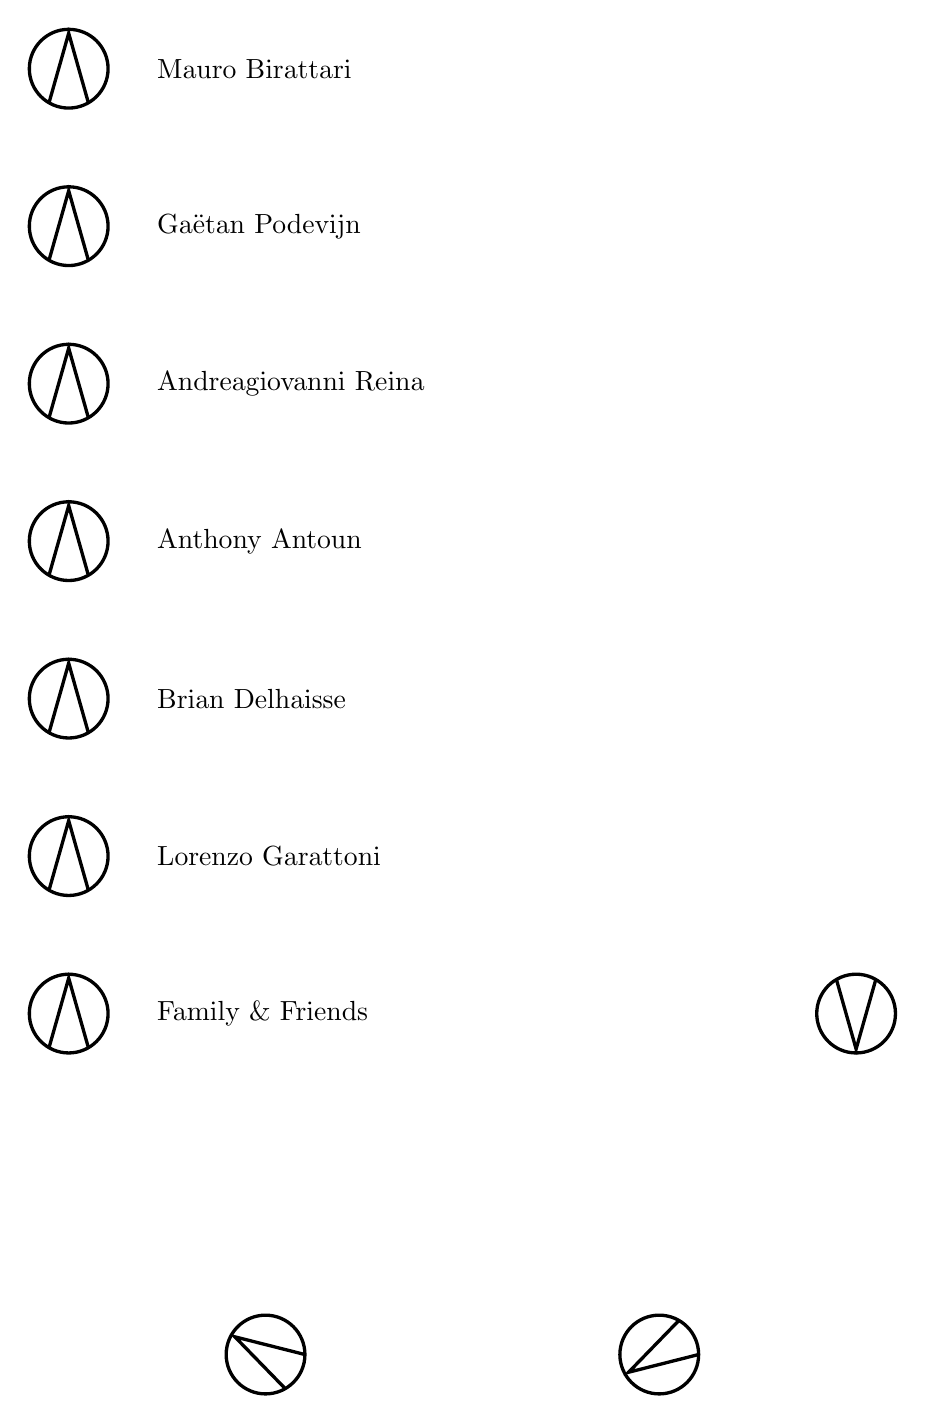
\begin{tikzpicture}
	%Mauro, Gaëtan, Giovanni, Anthony, Lorenzo, Brian, Family and friends.
	\epuck{-5}{12}
	\epuck{-5}{10}
	\epuck{-5}{8}
	\epuck{-5}{6}
	\epuck{-5}{4}
	\epuck{-5}{2}
	\epuck{-5}{0}
	\epuck[60]{-2.5}{-4.33}
	\epuck[120]{2.5}{-4.33}
	\epuck[180]{5}{0}
	
	\draw (-4,12) node[anchor=west] {Mauro Birattari};
	\draw (-4,10) node[anchor=west] {Gaëtan Podevijn};
	\draw (-4,8) node[anchor=west] {Andreagiovanni Reina};
	\draw (-4,6) node[anchor=west] {Anthony Antoun};
	\draw (-4,4) node[anchor=west] {Brian Delhaisse};
	\draw (-4,2) node[anchor=west] {Lorenzo Garattoni};
	\draw (-4,0) node[anchor=west] {Family \& Friends};
	
	\end{tikzpicture}
\end{figure}

\chapter{Résumé}
\chapter{Summary}
\tableofcontents
\listoffigures
\listoftables

\listoftodos

%%%%%%%%%%%%%%%%%%%%%%%%%%%%%%%%%%%%%%%%%%%%%%%%%%%%%%%
% TEXT
%%%%%%%%%%%%%%%%%%%%%%%%%%%%%%%%%%%%%%%%%%%%%%%%%%%%%%%
\mainmatter
\chapter{Introduction}

[I'll do this and this... blah blah blah...]

\begin{comment}
INTRO
Il faut respecter un fil conducteur dans la thèse. D'abord teaser le contenu dans l'introduction : "j'ai fait un super controller qui peut permettre à des robots de protéger un humain. Ca n'avait jamais été fait avant. J'utilise une swarm. J'ai de très bons résultats. On a testé avec des vrais robots, et l'humain est empêché d'accéder à des zones dangereuses.

STATE OF THE ART
Voici ce qui existe dans le domaine human - robot interaction. Rien de tout cela ne me satisfait et répond à mon problème.

Idem pour human - swarm interaction.

Je vais donc essayer de répondre au problème avec une nouvelle solution... Elle est meilleure que les autres pour ce problème car...

SOLUTION
Pour parvenir à mes fins, j'ai dû implémenter un controller. J'ai choisi virtual physics car ces avantages et inconvénients. C'est ce gars qui l'a inventé, et voici les travaux utilisant cette technique.

\end{comment}

As swarm robotic systems are mostly destined to operate on risky floors, unknown environment, it would seem logical to consider their application in exploration and/or protection missions. However, at the time of writing this thesis, we could not find any study on the subject. Exploration experiments never included a human, or other living organism. The object of this thesis is to address this lack of study by designing and implementing a protective behaviour executed by a robotic swarm.
	
	The human operator is here part of the swarm system. The swarm has to protect him by preventing him from going into dangerous areas, in the same way a group of bodyguards protects someone. The swarm has to follow the operator anywhere to ensure permanent protection.\\
	
	We believe this work to be important since it could lay the foundations of a new branch in swarm engineering: human protection, escort or swarm turn-by-turn navigation.

\chapter{State of the Art}
	
	In this section, we will discuss the problem that led to the creation of this thesis by first providing the reader with some general insight in the world of swarm robotics and swarm intelligence. Then we will focus on specific parts of these domains of study: feedbacks between human and single robot, and human and robots' swarm.
	
	\section{Human - Robot Interaction}
	
	[Work related to what I do (detect humans, protection, follow person). Conclude on why it cannot be applied to my problem.]

	\section{Swarm Robotics}
	
	[Flocking with a guide, and then Pattern Formation with a Guide. Work related to what I do. Conclude on why it cannot be applied to my problem. Make connections with this part later in the document. S'inspirer de Brambilla pour les flock et pattern.]
	
	This section and the next one are largely inspired by~\citet{brambilla2013swarm}, a reviewing article on swarm engineering. For \citet{csahin2005swarm}, swarm robotics is defined as \quot{the study of how large numbers of relatively simple physically embodied agents can be designed such that a desired collective behavior emerges from the local interactions among agents and between the agents and the environment}~\citep{csahin2005swarm}. Swarm robotics can be separated from other robotic studies by the following characteristics \citep{brambilla2013swarm}:
	
\begin{itemize}
\item Robots are \emph{autonomous}
\item Robots evolve \emph{in the environment} and can interact with it
\item Robots' interactions are \emph{local} (sensors and communications)
\item No \emph{centralised control} or \emph{global knowledge}
\item Robots \emph{cooperate} to achieve a certain goal
\end{itemize}

As in this field of study, one is always looking for \emph{robust}, \emph{scalable} and \emph{flexible} systems, the main source of inspiration is the group of social animals: ants, birds, fishes, ... When some of these simple animals gather in groups, they are able to perform tasks that could not be achieved individually (collective behaviour emerges from local interactions). Below are listed the definitions of these three terms \citep{brambilla2013swarm}:

\label{def:robustness_scalability_flexibility}
\begin{description}
\item[Robustness:] Resistance against \emph{loss of group entities}. One can increase it by adding redundancy or remove the need for a leader.
\item[Scalability:] Low variation in the performance of a system with respect to the \emph{size of the system}. It can be increased by encouraging local interactions, such as sensing and communications.
\item[Flexibility:] Low variation in the performance of a system with respect to the \emph{type of environment or the task}.
\end{description}

With these definitions in mind, we can explain swarm engineering as:

\quoto{Swarm engineering is an emerging discipline that aims at defining systematic and well founded procedures for modeling, designing, realizing, verifying, validating, operating, and maintaining a swarm robotics system.}{\cite{brambilla2013swarm}}

\citet{kazadi2000swarm} points out that \quot{to the swarm engineer, the important points in the design of a swarm are that the swarm will do precisely what it is designed to do, and that it will do so reliably and on time} \citep{kazadi2000swarm}.
	
	\subsection{Human - Robots Swarm Interaction}
	
	[Work related to what I do (detect humans, protection, follow person). Conclude on why it cannot be applied to my problem.]
	
	Human - Robotic swarm interaction is the study of how humans can interact with a swarm to control it and receive feedback from it \citep{brambilla2013swarm}. A proper feedback is needed by the operator in order to make the right decisions. Since swarms must ideally be autonomous and make decisions in a distributed way, it is difficult to insert a communication with a human operator in the system to gain control.\\
	
	Currently, little attention has been devoted to the study of the interaction between humans and robotic swarms, how one can send instructions and receive feedback. People investigating in the field encounter many difficulties, such as the difference of perspective between the swarm and the human operator (the human only observes the global collective behaviour, not the local interactions or individual behaviours driving the robots), the simplicity of the hardware found on the robots, or the efficient synthesis of all the information sent by the robots. All the existing types of interactions in the literature present a major disadvantage: they require an extra layer between the group of robots and the human. This requirement might not always be satisfied when we remember that swarms like this are mostly destined to evolve in an unknown environment. The monitoring equipment necessary to operate the swarm may not be safely deployed. Furthermore, a synthesis of all the local information pieces must be done in order to provide an understandable state of the system to the human. A supplementary step that involves modelling, additional overheads and perhaps heavy computations, and the gathering of all information at a central point (eliminating by the way the distributed and not centralised properties of the swarm system) \citep{podevijn2012self}.\\
	
	\citet{daily2003world} used a head-mounted display and augmented reality to add information right on top of the robot in the environment itself, suppressing the need for an additional display. \citet{baizid2009human} proposed a platform to interact with multiple robots simultaneously through a graphical user interface, or a head-mounted display, virtual reality etc. They also studied how virtual reality abstraction affected the human perception and cognitive capabilities, i.e, they created a virtual environment by filtering useless information. \citet{mclurkin2006speaking} developed an centralised graphical user interface taking inspiration from real-time strategy video games, where one must control armies. They also imagined a feedback approach based on LEDs and sounds. The robots transmit their internal state by applying to their LEDs and sound system a defined pattern, recognisable by the operator, now able to quickly understand the state of the swarm without looking at a supplementary interface.
	
	\citet{podevijn2012self} argue that self-organised mechanism, as those ruling the behaviour of the swarm, should be used to provide feedback to the operator. They suggest that the best entity which could communicate the status of the system and the whole swarm is the swarm itself. They performed experiments using colour feedback to distinguish different internal states and split the swarms into groups to tackle different tasks.\\
	
\begin{comment}
[Currently, only little research on feedback between human and robots swarms. That research is focused on interaction with an additional layer... Mostly unidirectional communication (human to robots). Need new types of interactions for new applications. Robots to human (guide). Write about article saying self-organised feedback is better.] \todo{Remove}
\end{comment}

	
		
		
	
	As swarm robotic systems are mostly destined to operate on risky floors, unknown environment, it would seem logical to consider their application in exploration and/or protection missions. However, at the time of writing this thesis, we could not find any study on the subject. Exploration experiments never included a human, or other living organism. The object of this thesis is to address this lack of study by designing and implementing a protective behaviour executed by a robotic swarm.
	
	The human operator is here part of the swarm system. The swarm has to protect him by preventing him from going into dangerous areas, in the same way a group of bodyguards protects someone. The swarm has to follow the operator anywhere to ensure permanent protection.\\
	
	We believe this work to be important since it could lay the foundations of a new branch in swarm engineering: human protection, escort or swarm turn-by-turn navigation.

%////////////////////////////////////////////////////////////
\chapter{An Escorting Swarm}
%////////////////////////////////////////////////////////////
\label{chap:escorting_swarm}

\begin{comment}
[\textcolor{red}{This is the core of the thesis. It must be a standalone. The reader must understand my work through the reading of this part only!} Explain the solution independently of the tools used to implement the solution. Make the reader understand that this problem is new.

On veut protéger un humain qui ne voit rien comme danger. Solution: un swarm de robots perçu par l'humain avec UN WEARABLE DEVICE (en parler après avoir mentionné le challenge correspondant).

Challenges: une fois qu'on connait la solution générale, parler des challenges, genre comment reconnaître un humain?]\\
\end{comment}


This chapter will explore the problem faced, and its solution, with a high level of abstraction. The next chapter will go deeper in the details and explain how everything was implemented.

	\section{The Problem}
	
	\begin{comment}
	[Human walking in unknown environment. Team to assist, perceive danger that the human cannot. Graphical example, human goes from A to B with dangers (keep it simple as demo). Write text about an image showing the problem. Mined field, real applications.]\\
	\end{comment}
	
	Since the early days, man has tried to explore new territories to expand their control and get a better understanding of the world surrounding them. Among those new landscapes, some were relatively safe and some were dangerous. To address this issue, we have invented armours, shield, and other kinds of protections. This work tries to contribute to the study of these solutions.\\
	
	To get a better insight, let us imagine a world where dangerous areas are circular. The human, as depicted on figure \ref{fig:unknown_environment}, must travel from point \emph{A} to \emph{B} without being hurt. The problem is that the human has no clue where the dangerous areas are. The person cannot perceive them. They could be radioactive areas, mine fields, or any other invisible threats. The protection created should prevent the user from going inside those areas.\\
	
	Exploration is not the only real application that comes into mind. Rescue in disaster areas would also benefit from it (evacuation of people to safe zones, etc). The system created should be able to constantly protect the person using it, and constantly provide feedback. It should be robust and fit to the destination environment.
	
%	\begin{figure}\centering
%		\begin{tikzpicture}
%			\draw [dashed] (0,0) circle [radius=1];
%			\draw (0,0) node[scale=2]{A};
%			
%			\draw [dashed] (10,10) circle [radius=1];
%			\draw (10,10) node[scale=2]{B};
%			
%			\draw [dashed, fill=red] (5,5) circle [radius=3];
%			\draw (5,5) node[scale=5]{!};
%			
%			\draw [->, very thick, green] (0,1.5) to [out=90,in=180] (8.5,10);
%			\draw [->, very thick, green] (1.5,0) to [out=0,in=270] (10,8.5);
%			\draw [->, very thick, red] (1.5, 1.5) -- (2.5,2.5);
%		\end{tikzpicture}
%	\end{figure}
	
	\begin{figure}\centering
		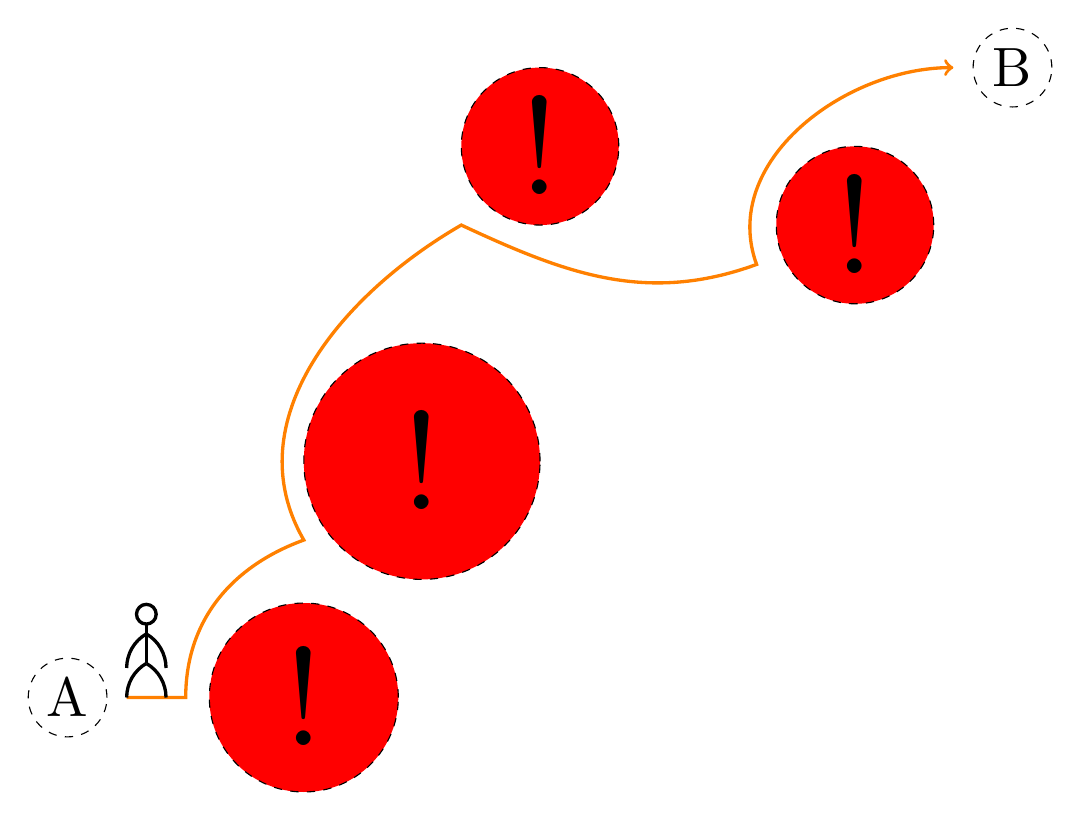
\begin{tikzpicture}
			\draw [dashed] (0,0) circle [radius=0.5];
			\draw (0,0) node[scale=2]{A};
			
			\draw [dashed] (12,8) circle [radius=0.5];
			\draw (12,8) node[scale=2]{B};
			
			\draw [dashed, fill=red] (3,0) circle [radius=1.2];
			\draw (3,0) node[scale=5]{!};
			
			\draw [dashed, fill=red] (4.5,3) circle [radius=1.5];
			\draw (4.5,3) node[scale=5]{!};
			
			\draw [dashed, fill=red] (6,7) circle [radius=1];
			\draw (6,7) node[scale=5]{!};
			
			\draw [dashed, fill=red] (10,6) circle [radius=1];
			\draw (10,6) node[scale=5]{!};
			
			\draw [->,very thick, orange] (0.75,0) to [out=0,in=180] (1.5,0) to [out=90,in=200] (3,2) to [out=120,in=-150] (5,6) to [out=-25, in=-160] (8.75,5.5) to [out=110, in=180] (11.25,8);
			
			\draw [very thick] (1,0.433) arc [radius=0.5, start angle=120, end angle=180];
			\draw [very thick] (1,0.433) arc [radius=0.5, start angle=60, end angle=0];
			\draw [very thick] (1,0.433) -- (1,0.933);
			\draw [very thick, fill=white] (1,0.433+0.625) circle [radius=0.125];
			\draw [very thick] (1,0.433+0.375) arc [radius=0.5, start angle=60, end angle=0];
			\draw [very thick] (1,0.433+0.375) arc [radius=0.5, start angle=120, end angle=180];
		\end{tikzpicture}
		
		\caption{Unknown Dangerous Environment}{This image illustrates an unknown environment, observed from above, in which a human must evolve while avoiding invisible dangerous areas. This figure represents a path to follow from \emph{A} to \emph{B} in a dangerous zone to stay safe. \emph{A} is the start location and \emph{B} is the goal. The red circles represent dangerous zones whose size can vary. This thesis explores a solution to guarantee safeness in such circumstances. Applications for this type of problems already exist: mine fields, radioactive areas, etc.}
		\label{fig:unknown_environment}
	\end{figure}
	
	
	\section{Solution}
	
	\begin{comment}
	[Solution at high level and the problems I will have to solve? Faire le lien avec flocking et pattern. \textcolor{red}{The swarm is extending the perception capabilities of the human.} Challenges.
	On a choisit d'utiliser des swarms car... Equidistance par rapport à l'humain. Carac du système. Pb pour détecter l'humain...avec solution. Agent de la swarm doit être capable de détecter le danger. Humain perçoit la swarm qui elle perçoit le danger.]
	\end{comment}
	
	The solution proposed involves the use of a swarm of robots. Swarm robotics seems fit to this kind of application, since it is compatible with unknown environments thanks to its flexible, robust and scalable characteristics \citep{brambilla2013swarm}. In case of failure of one or a few robots, the system would continue to provide sufficient performance thanks to its scalability and robustness.\\
	
	The swarm ideally forms a round shield around the user to ensure a 360° protection. All the robots try to stay at the same distance from each other and the person. To achieve this, the final solution relies on the pattern formation theory widely used in swarm robotics\todo{Parler du flocking et pattern.}. The corresponding techniques will be explained in the next chapter with more details. If the amount of robots is not high enough to form a complete circle, an arc is formed at the front to always shield the most critical zone.\\
	
	As seen on figure \ref{fig:swarm_preventing}, the robots in contact with a dangerous zone will reflect the danger through visual communication with the human. Here the robots turn red and stay on the boundary of the zone to prevent the user from getting into it. Since the human cannot see the danger, and only the robots can, we can see that the swarm is increasing the perception capabilities of the user.\\
		
	\begin{figure}\centering
		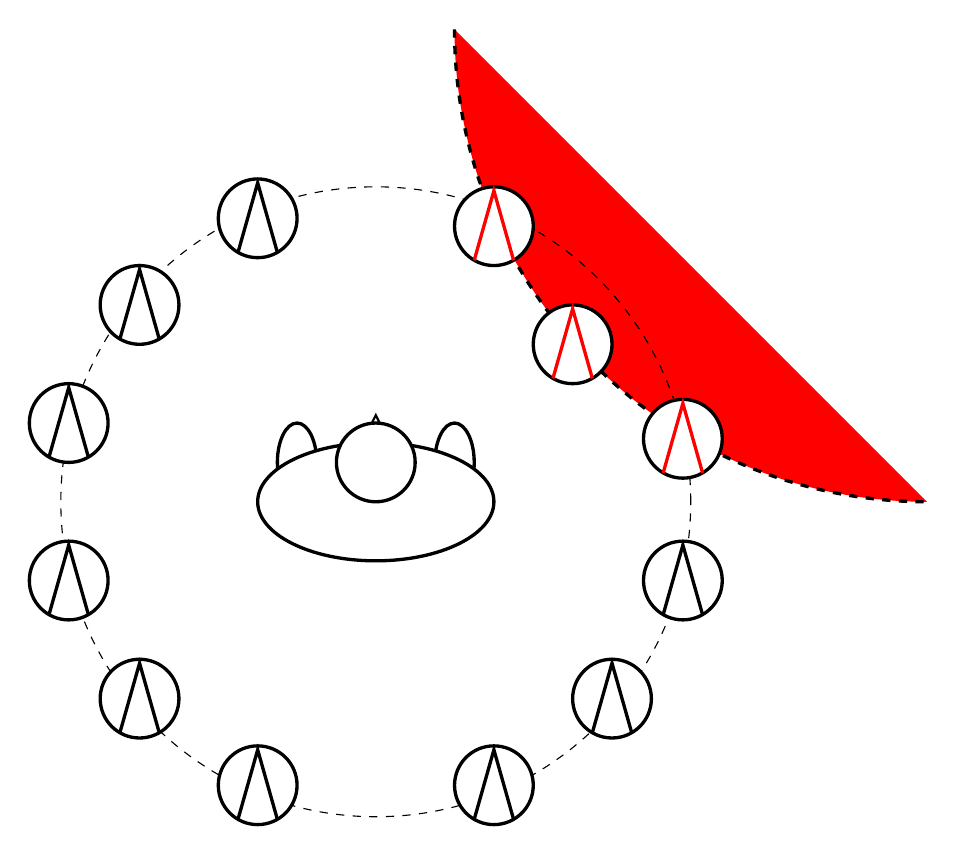
\begin{tikzpicture}
		
		%	\foreach \i in {\xMin,...,\xMax} {
		%        \draw [very thin,gray] (\i,\yMin) -- (\i,\yMax)  node [below] at (\i,\yMin) {$\i$};
		%    }
		%    \foreach \i in {\yMin,...,\yMax} {
		%        \draw [very thin,gray] (\xMin,\i) -- (\xMax,\i) node [left] at (\xMin,\i) {$\i$};
		%    }
			
			\draw [very thick, dashed, fill=red] (2,6) arc [radius=6, start angle=180, end angle=270];
			
			\draw [very thick, fill=white] (0,0.5) ellipse (0.25cm and 0.5cm);
			\draw [very thick, fill=white] (2,0.5) ellipse (0.25cm and 0.5cm);
			\draw [very thick, fill=white] (1,0) ellipse (1.5cm and 0.75cm);
			\draw [thick] (0.95,1) -- (1,1.1) -- (1.05,1);
			\draw [very thick, fill=white] (1,0.5) circle [radius=0.5cm];
			%\draw (1,-0.2) node [scale=2] {Human};
			
			\draw [dashed] (1,0) circle [radius=4];
			
			\epuckred{2.5}{3.5}
			\epuckred{3.5}{2}
			\epuckred{4.9}{0.8}
			\epuck{4.9}{-1}
			\epuck{4}{-2.5}
			\epuck{2.5}{-3.6}
			\epuck{-2.9}{-1}
			\epuck{-2}{-2.5}
			\epuck{-0.5}{-3.6}
			\epuck{-2.9}{1}
			\epuck{-2}{2.5}
			\epuck{-0.5}{3.6}
					
		\end{tikzpicture}
		
		\caption{Swarm Prevention}{This figure is a representation of a human helped by a swarm. The circles with a triangle inside are representations of a robot. The swarm tells the human that a dangerous zone is located at the front right by visual communication (here the robots change their colour to red). The swarm stays at the boundary to form a \enquote{shield}. The direction taken by each individual in the swarm is given by the triangle inside (here heading north).}
		\label{fig:swarm_preventing}
	\end{figure}
	
	One big issue that had to be resolved was the detection of the human by the robots. As \citet{podevijn2012self} suggested, the interface between the human and the robots swarm should be restricted to the strict minimum because in the field the infrastructure needed to operate the swarm might not be easy to build. The swarm should handle the communication on its own. Furthermore, any centralised control system would break the distributed and robust feature of swarm robotics. We thus imagined a wearable device that would allow the human to be recognised by the robots: a pair of shoes.\\
	
	\begin{figure}
		\begin{minipage}[c]{0.6\textwidth}
			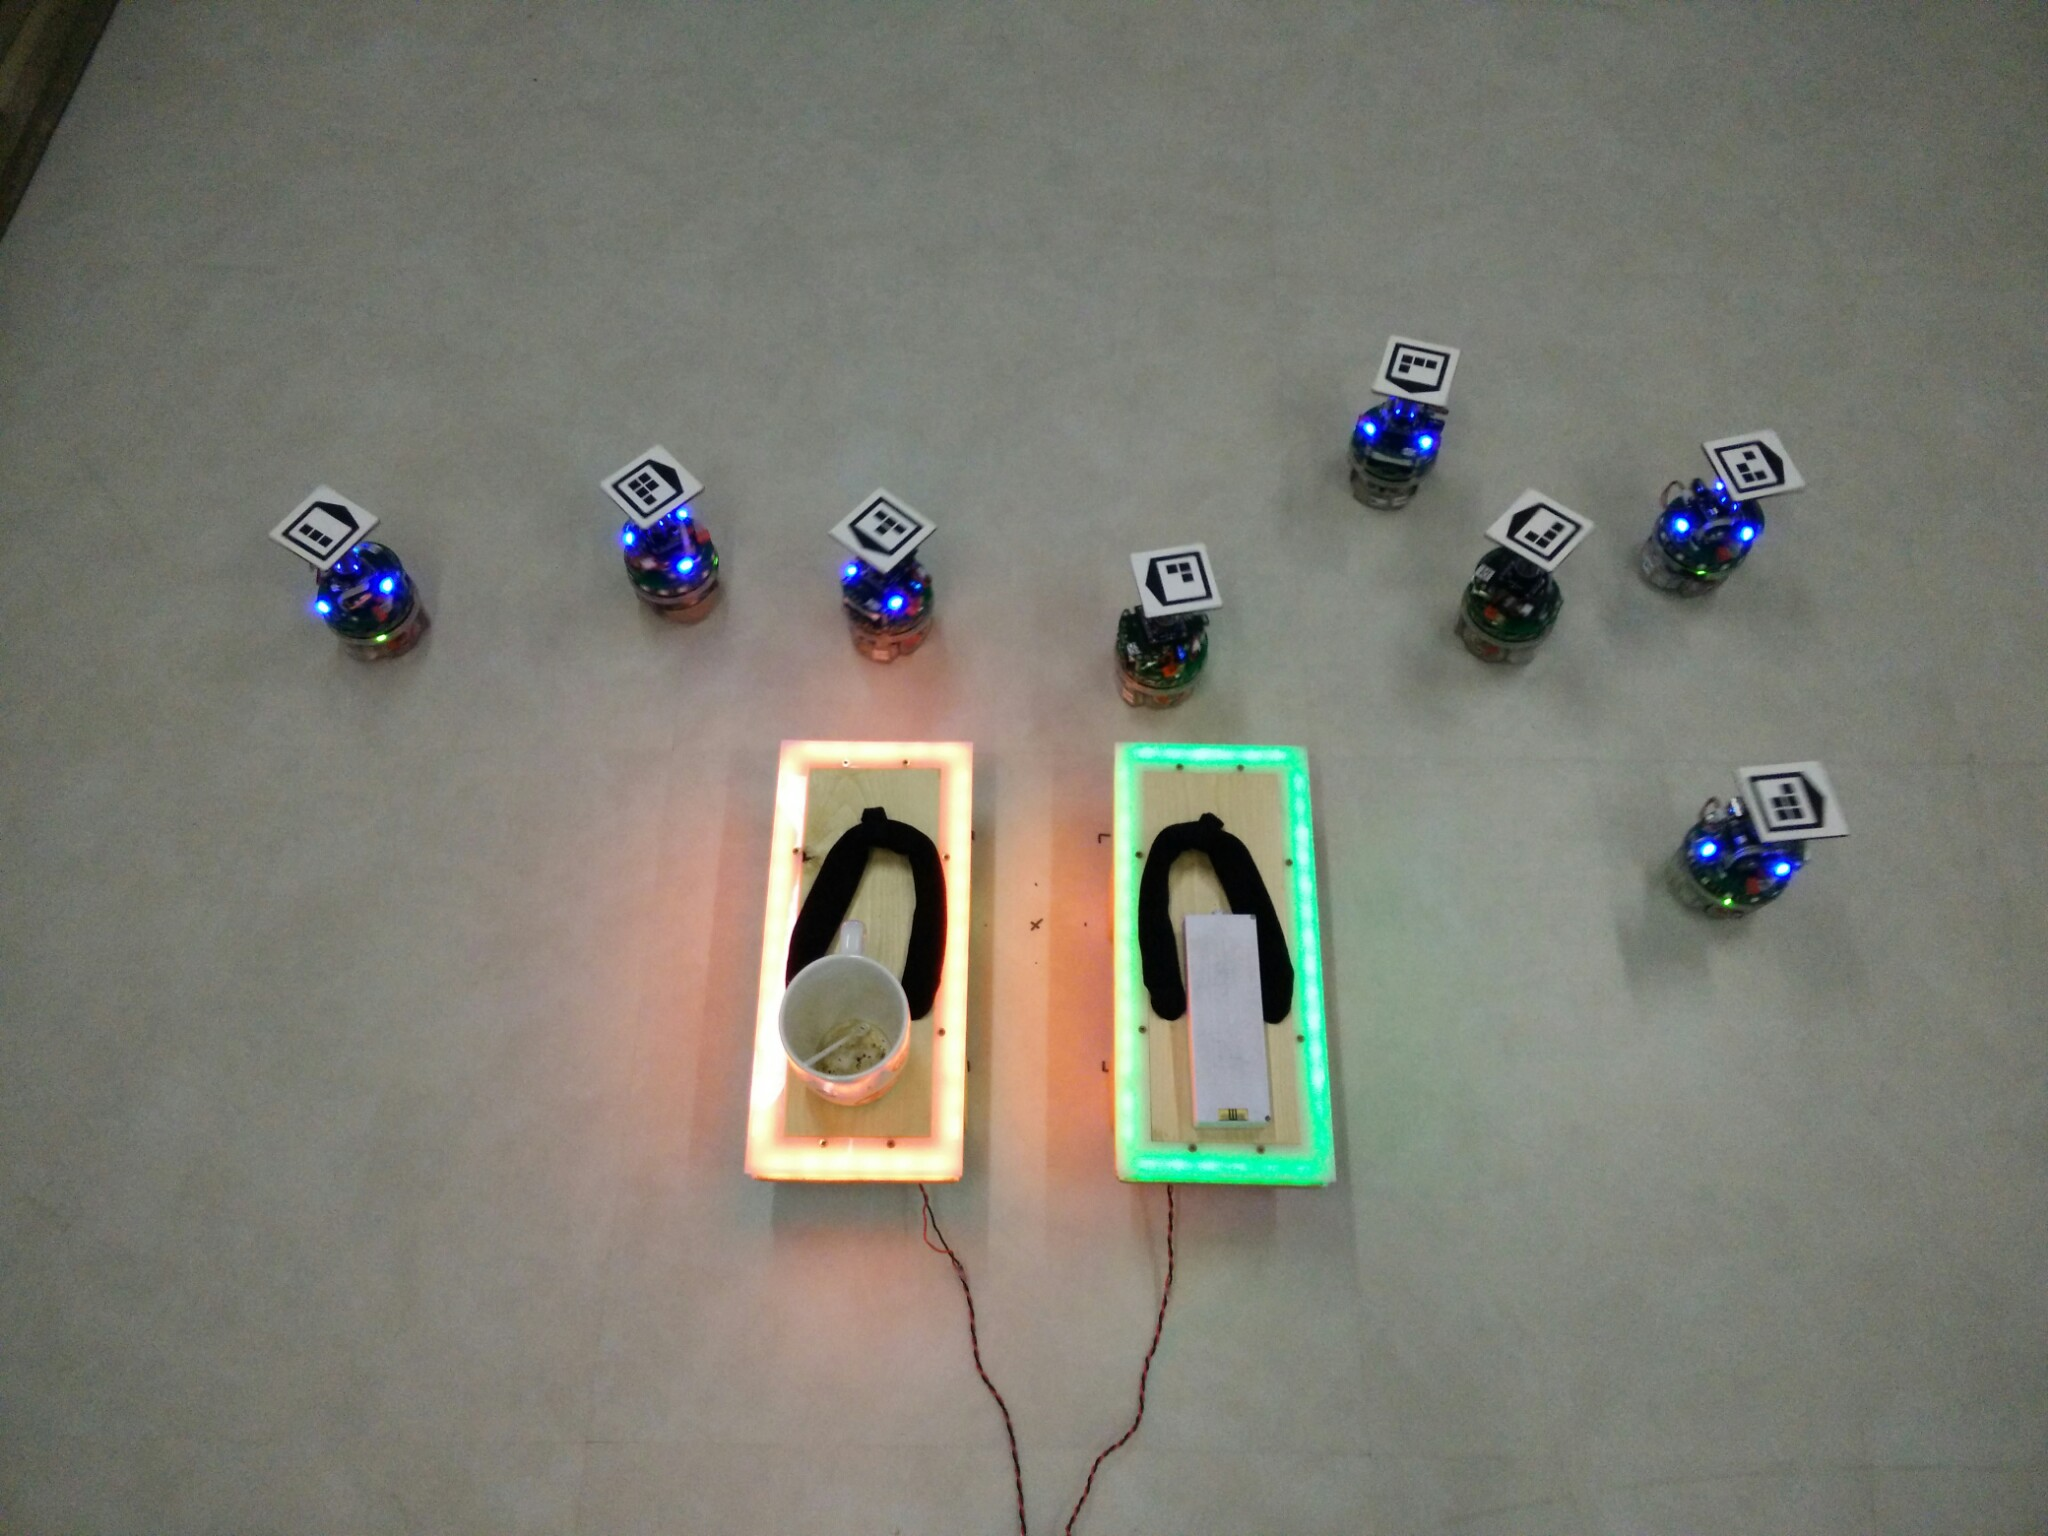
\includegraphics[trim=200px 300px 140px 300px, clip=true, height=5cm]{images/shoes.jpg}
		\end{minipage}
		\hfill
		\begin{minipage}[c]{0.39\textwidth}
			\hfill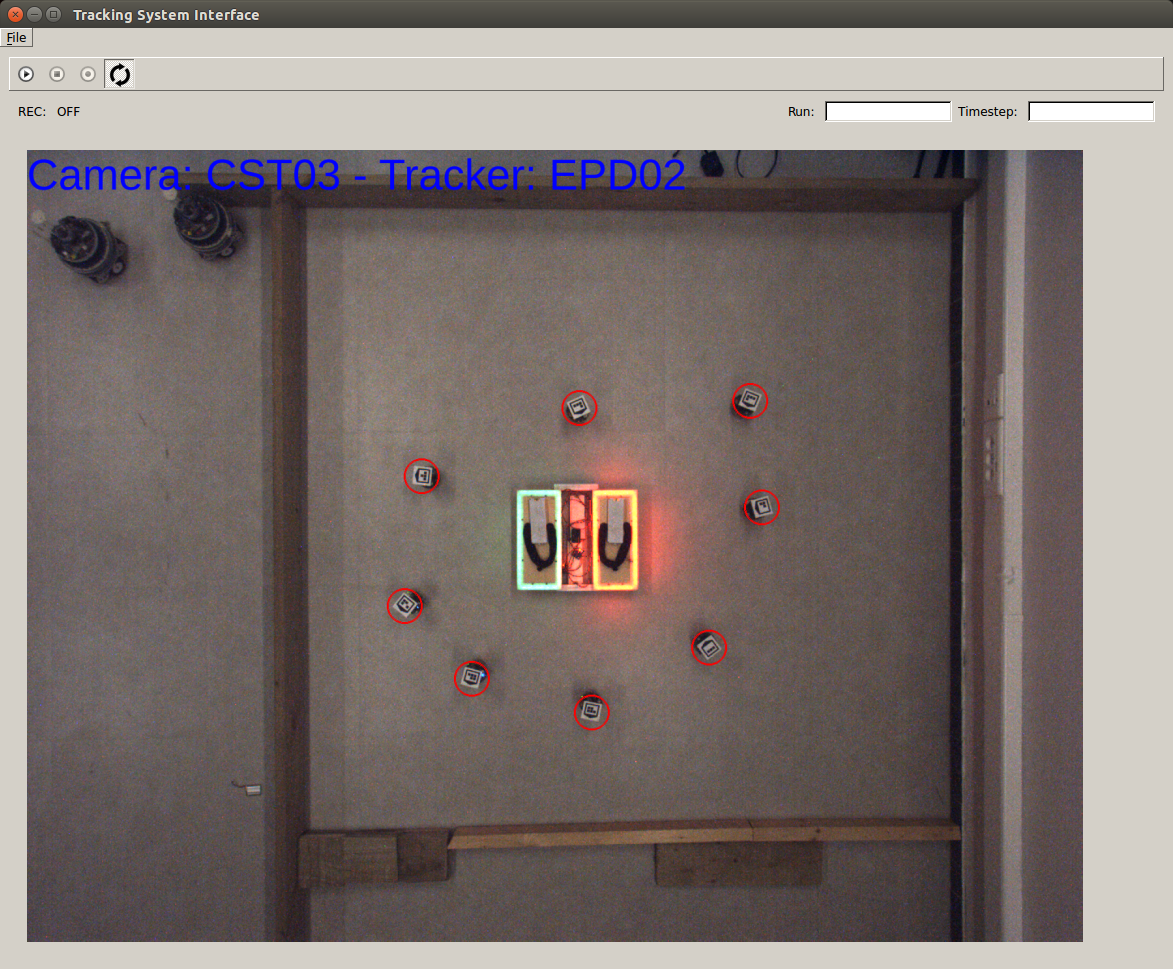
\includegraphics[trim=380px 230px 380px 360px, clip=true, height=5cm]{../Experiments/No_Human/6end.png}
		\end{minipage}				
		
		\caption{The Shoes}{This picture shows a prototype of the shoes viewed from above, and the robots interacting with it. The interaction is realised through the recognition of the colours, one for each shoe, indicating left or right side. This pair of shoes enables the robots to locate the user, allowing them to evolve at the target distance from him/her. On the left image, the robots are still in the process of placing themselves in a correct circle. The right image depicts the situation after a 3 minutes experiment where the robots were initially placed in lines around the shoes. Objects are put on the shoes to close the lights switch.}
		\label{fig:shoes}
	\end{figure}

The figure \ref{fig:shoes} illustrates the use of the shoes (no user is wearing them to increase visibility). On the left side, the robots have just recognised the shoes thanks to the LED system inside and begin to move to their target position. The right side is an example of one configuration obtained after 3 minutes, viewed from the ceiling tracking system.\\

This thesis objective was to present an innovative protection using swarm robotics. We consider the final protection robust. The results obtained at the end of the thesis with real robots will be detailed in the chapter \ref{chap:experiments}, but one can already say they are convincing. An article will be written during summertime to expose this research to the rest of the swarm robotics community.

%////////////////////////////////////////////////////////////
\chapter{Implementation}
%////////////////////////////////////////////////////////////

	This chapter details the solution to the given problem and all the choices that resulted in it. The explanation will take a top-down approach, first reviewing the hardware and the general code architecture. It will then go deeper in the details.\\
	
	The first question one could ask is: why swarm robotics for such an application? The answer to that question lays in section \ref{def:robustness_scalability_flexibility}. Robustness, scalability and flexibility are characteristics that make swarms of robots really interesting in unknown environments \citep{brambilla2013swarm}.\todo{Insert more justification?} In case one of the agents is broken, we do not want to see the whole system collapse and leave the human unattended. Flexibility guarantees that the solution will work in different conditions, environments, which is an advantage for exploration and rescue. In case of loss of robots, scalability would maintain the protection performance to an acceptable level.
	
	\section{The Hardware}
	
	As explained in chapter \ref{chap:escorting_swarm}, one of the main issue was to enhance the robots so they could detect the user and position themselves with respect to him without any large external equipment. Large external equipments are not recommended since in the targeted unknown environment they might not be usable. For example, one might use a tracking system to get the position of the robots in real time and communicate it to the robots for them to adjust their speed. In controlled environment, this may work very well, but in the field it would be difficult to access that knowledge. The following sections will go through the details of the robots we used to conduct our experiments, and the prototype enabling swarm control.
	
		\subsection{E-puck}
		
		The robotic platform chosen was the e-puck \citep{mondada2009puck}. The robot model was made for educational purposes.
		
		\subsection{E-geta} % Longer text than for e-puck because more important!
	
		[I will in this section describe the need for a device to detect a human and its development. What are the objectives of the hardware? The choices we made to get the final solution. How we built it. Calibration an adaptation process to make the current algorithm compatible with the new hardware. Where does the term come from?]
	
	
	\section{The Robot Behaviour}
			
	The final implementation is built on 2 layers. The upper layer is the state machine, having for each state a specific behaviour in the lower layer. Figure \ref{fig:state_machine} illustrates the whole structure of the upper layer. Only part of the states rely on virtual physics: \emph{Human} and \emph{Default}. The others simply link the sensor values to the wheels speed.\\
	
	The transitions without any number are taken without any condition, right after the corresponding behaviour has been applied (the time step period is over). One could see the 3 lowest states as sub-states of \emph{Normal}. At the beginning of each time step, if the controller is in the \emph{Normal} state, it has to choose between the 3 different sub-states. The conditions are listed with numbers in the figure \ref{fig:state_machine}.
	
	\begin{figure}[!h]\centering
		\begin{minipage}[c]{.49\textwidth}
			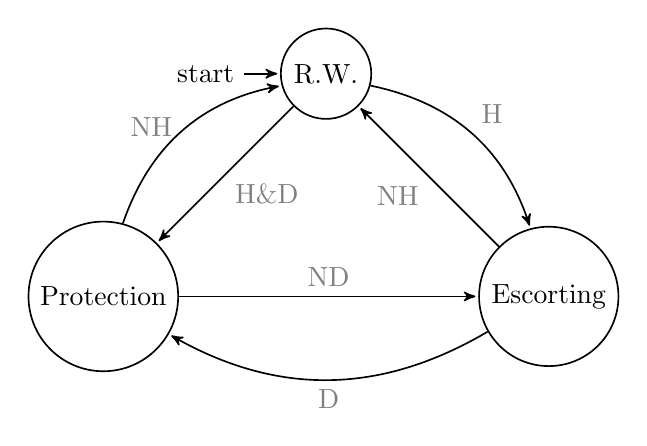
\begin{tikzpicture}[->, >=stealth', shorten >=1pt, auto, node distance=4cm, semithick]
				\node[initial,state] (RW)                    {R.W.};
		  		\node[state]         (E) [below right of=RW] {Escorting};
		  		\node[state]         (P) [below left of=RW] {Protection};
		  		
		  		\path	(RW)	 edge[bend left] node{\color{gray} H} (E)
		  				(RW)	 edge node{\color{gray} H\&D} (P)
		  				(E) edge node {\color{gray} NH}	(RW)
		  				(E) edge[bend left] node {\color{gray} D}	(P)
		  				(P) edge node {\color{gray} ND}	(E)
		  				(P) edge[bend left] node[yshift=-0.2cm] {\color{gray} NH}	(RW);

			\end{tikzpicture}
			
%			\resizebox{\textwidth}{!}{%
		  				
		\end{minipage}
		\hfill
		\begin{minipage}[c]{.49\textwidth}
		\resizebox{\textwidth}{!}{%
			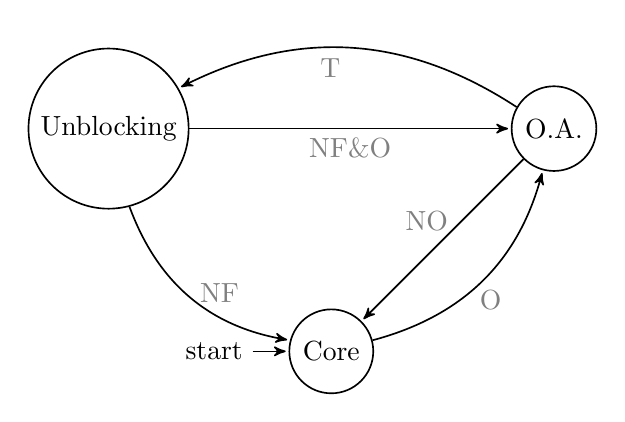
\begin{tikzpicture}[->, >=stealth', shorten >=1pt, auto, node distance=4cm, semithick]
				\node[initial,state] (C)                    {Core};
		  		\node[state]         (O) [above right of=C] {O.A.};
		  		\node[state]         (U) [above left of=C] {Unblocking};
		  		
		  		\path	(C)	edge[bend right] node[below,xshift=0.1cm]{\color{gray} O} (O)
		  				(O) edge node[above,xshift=-0.2cm] {\color{gray} NO}	(C)
		  				(O) edge[bend right] node {\color{gray} T}	(U)
		  				(U) edge node[below] {\color{gray} NF\&O}	(O)
		  				(U) edge[bend right] node[yshift=-0.2cm] {\color{gray} NF}	(C);

			\end{tikzpicture}}
		\end{minipage}
		
		\caption{State Machine of the Final Behaviour}{This figure is the visual representation of the state machine of the final behaviour. The left part is what could be called the \enquote{core} of the behaviour, while the right part would be considered as additions to enhance the behaviour. The core part of the state machine is present on the right since it is one of its constituents. The abbreviations R.W. and O.A. respectively mean \enquote{random walking} and \enquote{obstacle avoidance}. The labels next to each transition must be read as follows: H(uman), D(anger), O(bstacle), F(ront obstacle), T(hreshold crossed, stuck for too long and initiating rotation procedure to escape from the obstacles). N stands for the negation, so NH means \enquote{no human found}.}
		\label{fig:state_machine}
	\end{figure}
		
	
	
	The first step of the thesis is the design of the solution, to imagine how the system will look like and how we will implement it. The first choice faced was the overall behaviour of the swarm. How do the robots move around the human? What shape will they try to respect? This choice is important because it will define the overall look of the system.\\
	
	The first shape that intuitively comes in mind is the circle. The circle is the most elementary shape in geometry. It offers the best ratio:
	$$\frac{\mbox{Surface}}{\mbox{Perimeter}} = \frac{r}{2}~\mbox{, where r is the radius of the circle.}$$
	
	That means that fewer robots are needed for the same protected area, and more space for the human with a certain amount of robots. Luckily, it is also the easiest shape to realise in practice.
	
	\begin{figure}[!h]\centering
	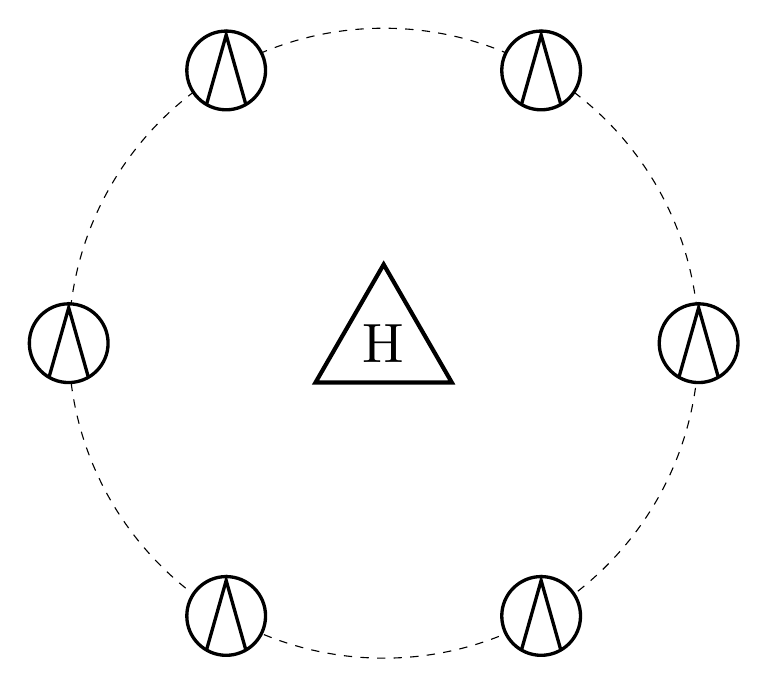
\begin{tikzpicture}
		\draw [dashed] (0,0) circle [radius=4];
		\epuck{4}{0}
		\epuck{2}{3.464}
		\epuck{-2}{3.464}
		\epuck{-4}{0}
		\epuck{-2}{-3.464}
		\epuck{2}{-3.464}
		
		\human{0}{0}
		%\draw (0,0) node[regular polygon,regular polygon sides=3,minimum height=2cm,minimum width=1cm,line width=1.5pt, draw] {\Huge{H}};
	\end{tikzpicture}
	\caption{Test}{Circle shape for the swarm to get the widest protected surface for a given amount of robots.}
	\label{fig:circle_shape}
	\end{figure}
	
		The figure \ref{fig:circle_shape} represents the kind of circle that we would like to get for 6 robots and 1 human in the centre.
		
	
	Section \ref{sec:virtual_physics} explained how the laws of physics can be used to design a behaviour. Intuitively, this method seemed the most appropriate to create a behaviour whose main feature is a \enquote{protection barrier} around a human. When it comes to pattern creation, people usually first consider using repulsive and attractive forces to make the robots automatically adjust their position with respect to others.\\
	
	Indeed, the laws of physics force the system to get to a state of minimum energy, i.e., to reach a global minimum of the potential function of the system. Since the force is proportional to the derivative of the corresponding potential, the minimum of the potential function means the disappearance of the forces. For the forces to disappear, every robot needs to be at the desired location.
	
	$$\vec{f} = -\vec{\nabla}P$$, P being the system's potential. The following sections will explain in detail the different potentials that were implemented to obtain the desired behaviour.
			
		In this section, the potentials are grouped by states in which they are used. Since virtual physics are used in only 2 states, we have only 2 groups.
		
			\paragraph{Human}
			
			The controller enters the \emph{Human} state at the beginning of the time step only if a human is found nearby. The complete potential for this state is the sum of 3 components: the \emph{human potential}, the \emph{gravity potential} and the \emph{agent repulsion potential}.
			
			\begin{enumerate}
				
				\item Human Potential
					
					\begin{figure}[!h]\centering
						\begin{tikzpicture}[xscale=0.2,yscale=0.2]
							\draw [<->] (0,5) -- (0,0) -- (70,0);
							\draw[blue,thick, domain=28:70] plot (\x, {-4*500/\x*((30/\x)^4-(30/\x)^2)});
							
							\foreach \x [evaluate=\x as \j using \x*10]in {0,...,6}
							    \draw (\j cm,5pt) -- (\j cm,-5pt) node[anchor=north] {$\j$};
							%\foreach \y in {0,1,2,3,4}
							%    \draw (1pt,\y cm) -- (-1pt,\y cm) node[anchor=east] {$\y$};
						\end{tikzpicture}
					\end{figure}
					
				\item Gravity Potential
				
				[Description of the evolution of the gravity potential.]
				
				\item Agent Repulsion Potential
				
				[Idem for agent repulsion pot.]
			\end{enumerate}
		
			\paragraph{Obstacle}
			
			[Idem for obstacle case.			
						
			\paragraph{Default}
			
			[Idem for the default state and potential.]
			
			\paragraph{Blocked}
			
			[Idem for blocked state.]
		

\chapter{Experiments}
\label{chap:experiments}
[\textcolor{red}{Explain very clearly both types of tests (no human/human.} ]

	\section{Characterisation of the System}
	[The measurements and the tests on the final behaviour.]

		\subsection{Metrics}
		
		[Metrics I will use. Their description. How I will compute them.]
		
			\paragraph{Correct Distance}
			
			[Do the robots respect the correct wanted distance?]
			
			\paragraph{Robot Density}
			
			[Do the robots surround the human correctly?]
			
			\paragraph{Time}
			
			[Do they do that in a relatively low amount of time?]
			
		\subsection{Set-up}
		
		[How I am performing my experiments.]
		
		\subsection{Analysis}
		
		[All the graphs we discussed about. The evolution of the error over time. The analysis of the behaviour on basis of the criteria we defined.]
		
	\section{Demonstration}
	
	[What demonstration was done with the device. Add pictures. Describe perfectly.]

\chapter{Conclusion}

[I've done this, this and this (~1/2 pages). (Intro: "I'll do this, this...) \textcolor{red}{Put sentences of type "so what?". Continuous text.}

	\paragraph{Future Works}
	[The future works that would be interesting from my point of view.]
	
		\subparagraph{Other Robots}
		\subparagraph{Guidance}
			
			\begin{description}
				\item[Zero Visibility Areas or Blind People:]
				\item[Human Motion Synchronisation:]
				\item[Vehicle Guidance:]
			\end{description}
			


\appendix

\chapter{The Complete State Machine}
\label{app:complete_state_machine}

\begin{figure}[!h]\centering
	\begin{minipage}[c]{.49\textwidth}
%			\begin{tikzpicture}[->, >=stealth', shorten >=1pt, auto, node distance=4cm, semithick]
%				\node[initial,state] (NORMAL)                    {Normal};
%		  		\node[state]         (OBS) [below left of=NORMAL] {Obstacle};
%		  		\node[state]         (HU) [below of=NORMAL] {Human};
%		  		\node[state]         (DEF) [below right of=NORMAL] {Default};
%		  		\node[state]         (BLOCK) [above of=NORMAL]       {Blocked};
%		  		
%		  		\path	(BLOCK)		edge		node					{\color{gray} 1}	(NORMAL)
%		  				(NORMAL)		edge		node[yshift=0.2cm]	{\color{gray} 2}	(OBS)
%		  				(NORMAL)		edge		node					{\color{gray} 3}	(HU)
%		  				(NORMAL)		edge		node	[yshift=-0.2cm]	{\color{gray} 4}	(DEF)
%		  				(OBS)		edge		[bend left]	node		{\color{gray} 5}	(BLOCK)
%		  				(OBS)		edge		[bend right]	node		{}				(NORMAL)
%		  				(HU)			edge		[bend right]	node		{}				(NORMAL)
%		  				(DEF)		edge		[bend right]	node		{}				(NORMAL);
%			\end{tikzpicture}
%			
		\resizebox{\textwidth}{!}{%
		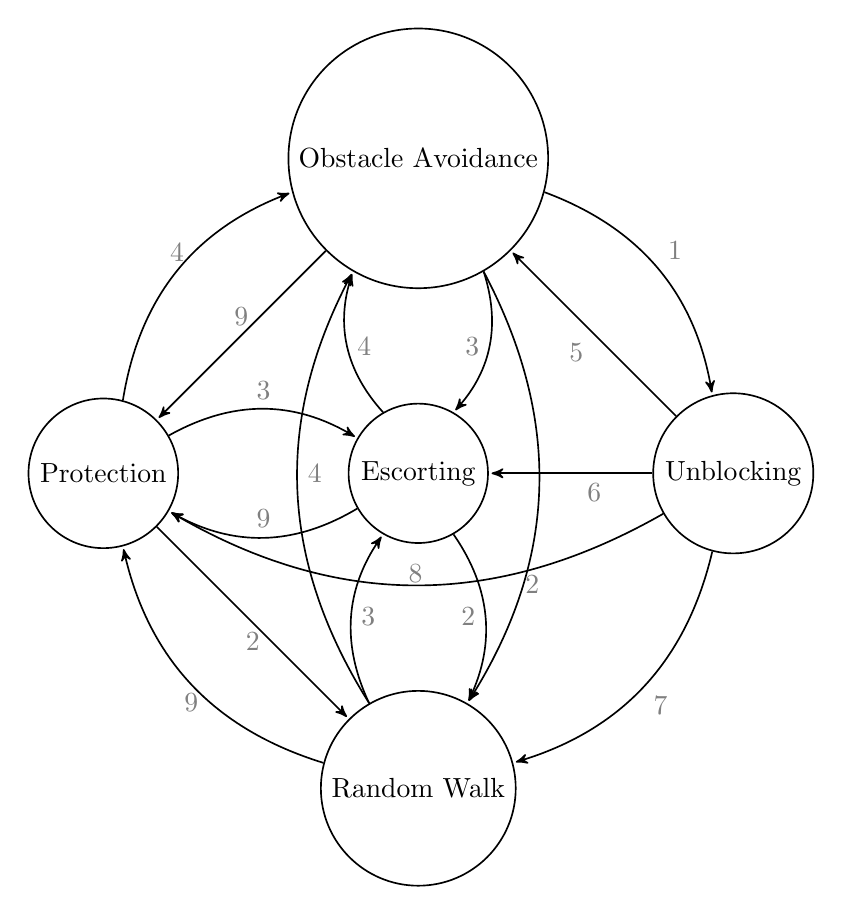
\begin{tikzpicture}[->, >=stealth', shorten >=1pt, auto, node distance=4cm, semithick]
	  		\node[state]         (OBS)					{Obstacle Avoidance};
	  		\node[state]         (HU) [below of=OBS]		{Escorting};
	  		\node[state]         (DEF) [below of=HU]		{Random Walk};
	  		\node[state]         (BLOCK) [right of=HU]	{Unblocking};
	  		\node[state]         (DANGER) [left of=HU]	{Protection};
	  		
	  		\path	(OBS)		edge	[bend left]	node		{\color{gray} 1}	(BLOCK)
	  				(OBS)		edge	[bend left]	node[yshift=-1.2cm, xshift=-0.3cm]		{\color{gray} 2}				(DEF)
	  				(OBS)		edge	[bend left]	node	[left]	{\color{gray} 3}				(HU)
	  				(HU)			edge	[bend left]	node[right]		{\color{gray} 4}				(OBS)
	  				(HU)			edge	[bend left]	node	[left]	{\color{gray} 2}				(DEF)
	  				(DEF)		edge	[bend left]	node[right]		{\color{gray} 3}				(HU)
	  				(DEF)		edge	[bend left]	node	[right, yshift=0.2cm]	{\color{gray} 4}				(OBS)
	  				(BLOCK)		edge				node		{\color{gray} 5}				(OBS)
	  				(BLOCK)		edge				node	[xshift=0.3cm]	{\color{gray} 6}				(HU)
	  				(BLOCK)		edge	[bend left]			node		{\color{gray} 7}				(DEF)
	  				(BLOCK)		edge	[bend left, above]	node[yshift=-0.1cm]		{\color{gray} 8}				(DANGER)
	  				(HU)		edge	[bend left, above]	node		{\color{gray} 9}				(DANGER)
	  				(DANGER)	 edge[bend left, above] node{\color{gray} 3} (HU)
	  				(DANGER)	 edge[bend left, above] node{\color{gray} 4} (OBS)
	  				(OBS)	 edge[above] node{\color{gray} 9} (DANGER)
	  				(DANGER)	 edge[below] node{\color{gray} 2} (DEF)
	  				(DEF)	 edge[bend left, below] node{\color{gray} 9} (DANGER);
	  				
		\end{tikzpicture}
		}
	\end{minipage}
	\hfill
	\begin{minipage}[c]{.49\textwidth}
		\small\sffamily
		
		\begin{enumerate}
			\item Amount of direction change (left/right) while having an obstacle around reaches a threshold.
			\item No human \& no obstacle.
			\item No obstacle \& human \& no danger.
			\item Obstacle.
			\item No front obstacle \& obstacle elsewhere.
			\item No front obstacle \& human \& no danger.
			\item No front obstacle \& no human \& no obstacle.
			\item No front obstacle \& human \& danger.
			\item No obstacle \& human \& danger.

			\end{enumerate}

%			\begin{enumerate}
%				\item No more obstacle in front.
%				\item Obstacle found around the robot.
%				\item Human found around the robot.
%				\item Neither of the previous criteria met.
%				\item Amount of direction change (left/right) while having an obstacle around reaches a threshold.
%			\end{enumerate}
	\end{minipage}
	
	\caption{State Machine of the Final Behaviour}{This figure is the visual representation of the state machine of the final behaviour. On the left, the states and their connections are drawn. On the right, the information on the conditions needed to take the transitions are listed.}
	\label{fig:state_machine}
\end{figure}

\chapter{E-puck}

\chapter{ARGoS}

\chapter{Arena Tracking System}

\chapter{Range and Bearing}

\chapter{Omnidirectional Camera}

\chapter{Controller Code}

\chapter{MATLAB Scripts Code}

\chapter{Human Detection Devices Blueprints}

\backmatter
\newpage

%%%%%%%%%%%%%%%%%%%%%%%%%%%%%%%%%%%%%%%%%%%%%%%%%%%%%%%
% BIBLIOGRAPHY
%%%%%%%%%%%%%%%%%%%%%%%%%%%%%%%%%%%%%%%%%%%%%%%%%%%%%%%

\begin{filecontents}{thesis.bib}
%http://en.wikibooks.org/wiki/LaTeX/Bibliography_Management

@inproceedings{podevijn2012self,
  title={Self-organised feedback in human swarm interaction},
  author={Podevijn, Ga{\"e}tan and O’Grady, Rehan and Dorigo, Marco},
  booktitle={Proceedings of the workshop on robot feedback in human-robot interaction: how to make a robot readable for a human interaction partner (Ro-Man 2012)},
  year={2012}
}

@incollection{podevijn2014gesturing,
  title={Gesturing at subswarms: Towards direct human control of robot swarms},
  author={Podevijn, Ga{\"e}tan and O’Grady, Rehan and Nashed, Youssef SG and Dorigo, Marco},
  booktitle={Towards Autonomous Robotic Systems},
  pages={390--403},
  year={2014},
  publisher={Springer}
}

@article{brambilla2013swarm,
  title={Swarm robotics: a review from the swarm engineering perspective},
  author={Brambilla, Manuele and Ferrante, Eliseo and Birattari, Mauro and Dorigo, Marco},
  journal={Swarm Intelligence},
  volume={7},
  number={1},
  pages={1--41},
  year={2013},
  publisher={Springer}
}

@incollection{csahin2005swarm,
  title={Swarm robotics: From sources of inspiration to domains of application},
  author={{\c{S}}ahin, Erol},
  booktitle={Swarm robotics},
  pages={10--20},
  year={2005},
  publisher={Springer}
}

@phdthesis{kazadi2000swarm,
  title={Swarm engineering},
  author={Kazadi, Sanza T},
  year={2000},
  school={California Institute of Technology}
}

@book{minsky1967computation,
  title={Computation: finite and infinite machines},
  author={Minsky, Marvin L},
  year={1967},
  publisher={Prentice-Hall, Inc.}
}

@article{granovetter1978threshold,
  title={Threshold models of collective behavior},
  author={Granovetter, Mark},
  journal={American journal of sociology},
  pages={1420--1443},
  year={1978},
  publisher={JSTOR}
}

@inproceedings{bonabeau1997adaptive,
  title={Adaptive Task Allocation Inspired by a Model of Division of Labor in Social Insects.},
  author={Bonabeau, Eric and Sobkowski, Andrej and Theraulaz, Guy and Deneubourg, Jean-Louis},
  booktitle={BCEC},
  pages={36--45},
  year={1997}
}

@article{bachrach2010composable,
  title={Composable continuous-space programs for robotic swarms},
  author={Bachrach, Jonathan and Beal, Jacob and McLurkin, James},
  journal={Neural Computing and Applications},
  volume={19},
  number={6},
  pages={825--847},
  year={2010},
  publisher={Springer}
}

@article{wolpert1999introduction,
  title={An introduction to collective intelligence},
  author={Wolpert, David H and Tumer, Kagan},
  journal={arXiv preprint cs/9908014},
  year={1999}
}

@article{abbott2006emergence,
  title={Emergence explained: Abstractions: Getting epiphenomena to do real work},
  author={Abbott, Russ},
  journal={Complexity},
  volume={12},
  number={1},
  pages={13--26},
  year={2006},
  publisher={Wiley Online Library}
}

@article{pinciroli2012argos,
  title={{ARGoS}: a Modular, Parallel, Multi-Engine Simulator for Multi-Robot Systems},
  author={Carlo Pinciroli and Vito Trianni and Rehan O'Grady and Giovanni Pini and Arne Brutschy and Manuele Brambilla and Nithin Mathews and Eliseo Ferrante and Gianni {Di Caro} and Frederick Ducatelle and Mauro Birattari and Luca Maria Gambardella and Marco Dorigo},
  journal={Swarm intelligence},
  volume={6},
  number={4},
  pages={271--295},
  year={2012},
  publisher={Springer},
  address = {Berlin, Germany}
}

@inproceedings{daily2003world,
  title={World embedded interfaces for human-robot interaction},
  author={Daily, Mike and Cho, Youngkwan and Martin, Kevin and Payton, Dave},
  booktitle={System Sciences, 2003. Proceedings of the 36th Annual Hawaii International Conference on},
  pages={6--pp},
  year={2003},
  organization={IEEE}
}

@incollection{baizid2009human,
  title={Human multi-robots interaction with high virtual reality abstraction level},
  author={Baizid, Khelifa and Li, Zhao and Mollet, Nicolas and Chellali, Ryad},
  booktitle={Intelligent Robotics and Applications},
  pages={23--32},
  year={2009},
  publisher={Springer}
}

@inproceedings{mclurkin2006speaking,
  title={Speaking Swarmish: Human-Robot Interface Design for Large Swarms of Autonomous Mobile Robots.},
  author={McLurkin, James and Smith, Jennifer and Frankel, James and Sotkowitz, David and Blau, David and Schmidt, Brian},
  booktitle={AAAI Spring Symposium: To Boldly Go Where No Human-Robot Team Has Gone Before},
  pages={72--75},
  year={2006}
}

@inproceedings{mondada2009puck,
  title={The e-puck, a robot designed for education in engineering},
  author={Mondada, Francesco and Bonani, Michael and Raemy, Xavier and Pugh, James and Cianci, Christopher and Klaptocz, Adam and Magnenat, Stephane and Zufferey, Jean-Christophe and Floreano, Dario and Martinoli, Alcherio},
  booktitle={Proceedings of the 9th conference on autonomous robot systems and competitions},
  volume={1},
  number={LIS-CONF-2009-004},
  pages={59--65},
  year={2009},
  organization={IPCB: Instituto Polit{\'e}cnico de Castelo Branco}
}

\end{filecontents}

%\nocite{*}
\bibliographystyle{plainnat}
\bibliography{thesis}

\end{document}
